\begin{pages}
    \begin{Rightside}
    \selectlanguage{greek}
        \beginnumbering
        \pstart[
        			\chapter{Ὁ παντοκράτωρ ἐπὶ τοῦ θρόνου αὐτοῦ}
        			\markboth{The Almighty Sitting upon His Throne}
				]
		Μετὰ ταῦτα εἶδον, καὶ ἰδοὺ θύρα ἠνεῳγμένη ἐν τῷ οὐρανῷ, καὶ ἡ φωνὴ ἡ πρώτη ἣν ἤκουσα ὡς σάλπιγγος λαλούσης μετ’ ἐμοῦ, λέγων Ἀνάβα ὧδε, καὶ δείξω σοι ἃ δεῖ γενέσθαι μετὰ ταῦτα. εὐθέως ἐγενόμην ἐν Πνεύματι· καὶ ἰδοὺ θρόνος ἔκειτο ἐν τῷ οὐρανῷ, καὶ ἐπὶ τὸν θρόνον καθήμενος, καὶ ὁ καθήμενος ὅμοιος ὁράσει λίθῳ ἰάσπιδι καὶ σαρδίῳ, καὶ ἶρις κυκλόθεν τοῦ θρόνου ὅμοιος ὁράσει σμαραγδίνῳ. καὶ κυκλόθεν τοῦ θρόνου θρόνους εἴκοσι τέσσαρας, καὶ ἐπὶ τοὺς θρόνους εἴκοσι τέσσαρας πρεσβυτέρους καθημένους περιβεβλημένους ἐν ἱματίοις λευκοῖς, καὶ ἐπὶ τὰς κεφαλὰς αὐτῶν στεφάνους χρυσοῦς. καὶ ἐκ τοῦ θρόνου ἐκπορεύονται ἀστραπαὶ καὶ φωναὶ καὶ βρονταί· καὶ ἑπτὰ λαμπάδες πυρὸς καιόμεναι ἐνώπιον τοῦ θρόνου, ἅ εἰσιν τὰ ἑπτὰ Πνεύματα τοῦ Θεοῦ· καὶ ἐνώπιον τοῦ θρόνου ὡς θάλασσα ὑαλίνη ὁμοία κρυστάλλῳ·
		\pend
		\pstart
		καὶ ἐν μέσῳ τοῦ θρόνου καὶ κύκλῳ τοῦ θρόνου τέσσερα ζῷα γέμοντα ὀφθαλμῶν ἔμπροσθεν καὶ ὄπισθεν. καὶ τὸ ζῷον τὸ πρῶτον ὅμοιον λέοντι, καὶ τὸ δεύτερον ζῷον ὅμοιον μόσχῳ, καὶ τὸ τρίτον ζῷον ἔχων τὸ πρόσωπον ὡς ἀνθρώπου, καὶ τὸ τέταρτον ζῷον ὅμοιον ἀετῷ πετομένῳ. καὶ τὰ τέσσερα ζῷα, ἓν καθ’ ἓν αὐτῶν ἔχων ἀνὰ πτέρυγας ἕξ, κυκλόθεν καὶ ἔσωθεν γέμουσιν ὀφθαλμῶν· καὶ ἀνάπαυσιν οὐκ ἔχουσιν ἡμέρας καὶ νυκτὸς λέγοντες Ἅγιος ἅγιος ἅγιος Κύριος ὁ Θεός ὁ Παντοκράτωρ, ὁ ἦν καὶ ὁ ὢν καὶ ὁ ἐρχόμενος. 
		\pend
		\pstart
		Καὶ ὅταν δώσουσιν τὰ ζῷα δόξαν καὶ τιμὴν καὶ εὐχαριστίαν τῷ καθημένῳ ἐπὶ τῷ θρόνῳ τῷ ζῶντι εἰς τοὺς αἰῶνας τῶν αἰώνων, πεσοῦνται οἱ εἴκοσι τέσσαρες πρεσβύτεροι ἐνώπιον τοῦ καθημένου ἐπὶ τοῦ θρόνου, καὶ προσκυνήσουσιν τῷ ζῶντι εἰς τοὺς αἰῶνας τῶν αἰώνων, καὶ βαλοῦσιν τοὺς στεφάνους αὐτῶν ἐνώπιον τοῦ θρόνου, λέγοντες Ἄξιος εἶ, ὁ Κύριος καὶ ὁ Θεὸς ἡμῶν, λαβεῖν τὴν δόξαν καὶ τὴν τιμὴν καὶ τὴν δύναμιν, ὅτι σὺ ἔκτισας τὰ πάντα, καὶ διὰ τὸ θέλημά σου ἦσαν καὶ ἐκτίσθησαν.
		\pend
        \endnumbering
    \end{Rightside}
    \begin{Leftside}
        \beginnumbering
        \pstart[
        			\chapter{The Almighty Sitting upon His Throne}
				]
		After this I saw — and look! — a door having been opened in Heaven and the first voice I heard — (which spoke) like a trumpet — was speaking to me, saying, “Come up here and I will show you what must happen hereafter. Immediately I was in Spirit, and look! A throne (chair) placed within Heaven and someone was sitting on it; and He who was sitting on it was in appearance like a jasper and carnelian stone and a rainbow was around the throne, which looked as if it was made out of emeralds. And around the throne were (another) twenty-four thrones and upon those thrones were sitting twenty-four elders, (all) clad in white garments and upon their heads were golden crowns. And from the throne (there) came forth (bolts of) lightning, voices and thunder; and (there were) seven flaming torches burning before the throne which were the seven Spirits of God; and (the region) before the throne (was) as the Sea made of glass, like a crystal.
		\pend
		\pstart
		And in the middle of the throne and around the throne (there were) four living creatures, covered with eyes from back to front. And the first creature was like a lion, and the second creature was like a bull and the third creature had the head of a human, and the fourth creature was like a flying eagle. And the four creatures each had six wings (which) were filled with eyes around and within. And without a break — day and night — they were saying, “Holy, holy, holy (is the) Lord God, the Almighty, who was and is and who will come.”
		\pend
		\pstart
		Whenever the creatures give glory, honour and thanks to Him who sits upon the throne — He who will live into the eternity of eternities —, the twenty-four elders fall before the One sitting upon the throne and worship Him who lives into the eternity of eternities. And they throw their crowns before the throne, saying, “You are worthy, our Lord and God, of taking the glory, honour and power, for You created (the) everything; and through Your wish we were and were created.”
		\pend
        \endnumbering
    \end{Leftside}

\end{pages} 
\Pages

\clearpage
\thispagestyle{empty}
\null\vfill
\settowidth\longest{\huge\itshape […] and when I turned around I saw}
\begin{center}
\parbox{\longest}{%
  \raggedright{\huge\itshape%
    ``[…] A throne (chair) placed within Heaven and someone was sitting on it […]'' \par\bigskip
  }
  \raggedleft\Large\MakeUppercase{``Господь Вседержитель'' — Nikolay Koshelev, 1874}\par%
}
\vfill\vfill
\clearpage\newpage
\end{center}
\newpage
\thispagestyle{empty}
\begin{center}
	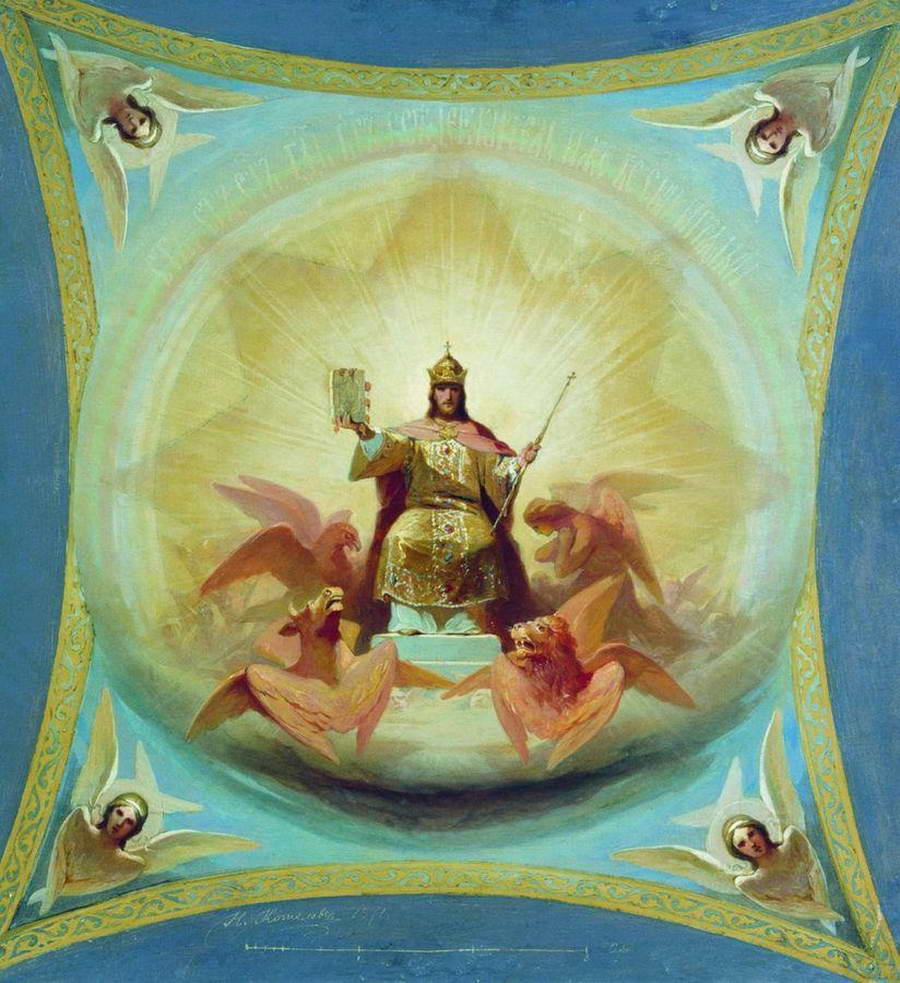
\includegraphics[width=1\textwidth]{images/illustrations/christpantokrator.jpg}
\end{center}